\chapter{Основной анализ}\label{ch:ch3}

В данной главе будут описаны результаты эмпирического анализа ценовых тенденций в российской экономике на основе собранных данных по ценам онлайн-ритейлеров.

\section{Описание данных}\label{sec:ch3/sec1}

При проектировании процесса сбора данных мы также старались придерживаться принципов, описанных в работе \cite{cavallo2016billion}. Прежде всего стоит отметить, что, аналогично подходу из упомянутой работы мы сосредоточились на сборе данных с сайтов самих магазинов, а не с сайтов-агрегаторов (или маркетплейсов). Этот подход оказался технически более сложным, но обеспечивающим актуальность цен и исключающим ошибки в других характеристиках, связанных с товаром.

Методика сбора данных состояла из нескольких этапов. На первом этапе были определены необходимые для последующего анализа товары и услуги. Следует отметить, что рынок онлайн-ритейла несмотря на свой бурный рост все еще ограничен с точки зрения географии и представленности различных товаров и услуг, что наложило отпечаток на характеристики выборки.

Мы отобрали ритейлеров, продающих товары как через интернет, так и в традиционных точках продаж. Лишь небольшая часть выбранных ритейлеров специализируется исключительно на онлайн-торговле. При выборе ритейлеров мы ориентировались на следующие критерии:
\begin{itemize}
	\item занимаемая доля рынка;
	\item охват по регионам;
	\item количество охватываемых ритейлером категорий продуктов.
\end{itemize}
Продовольственные и непродовольственные ритейлеры представлены крупнейшими онлайн-ритейлерами в своих сферах:
В качестве представителей продуктовых ритейлеров были отобраны следующие:

1) гипермаркет «Перекресток» (после 2021 г. - "Впрок");
2) гипермаркет «Глобус»;
3) гипермаркет «Окей»;
4) интернет-гипермаркет «Утконос».

В качестве представителей непродовольственных ритейлеров были выбраны:
1) интернет-магазин «Lamoda»;
2) интернет-магазин «Ozon.ru»;
3) интернет-магазин «Piluli.ru».

Сфера услуг представлена несколькими местными игроками рынка, которые специализируются на пассажирских перевозках, связи, жилищно-коммунальном хозяйстве, а также рядом небольших компаний, предлагающих услуги по ремонту обуви, посещению бани и парикмахерским услугам.

Несмотря на ограниченную географию сбора данных — Москва и Московский регион — полученная информация является достаточно репрезентативной. Например, в 2021 году доля «Впрок» составила 4,5\% от общего объема интернет-торговли в Москве~\cite{X5DigitalSales2021}, а «Ozon.ru» по состоянию на 2021 год занимал второе место среди крупнейших интернет-ритейлеров России~\cite{Top100Ecommerce2021}.

С сайтов интернет-ритейлеров нами извлекались различные характеристики товаров. Специальный скрипт, написанный на языке Python, запускался на ежедневной основе и сканировал разметку продуктовых страниц с товарами, представленными на сайтах онлайн-ритейлеров (пример части продуктовой страницы представлен на рис.~\cref{fig:example_product}).

\begin{figure}[ht]
	\centerfloat{
		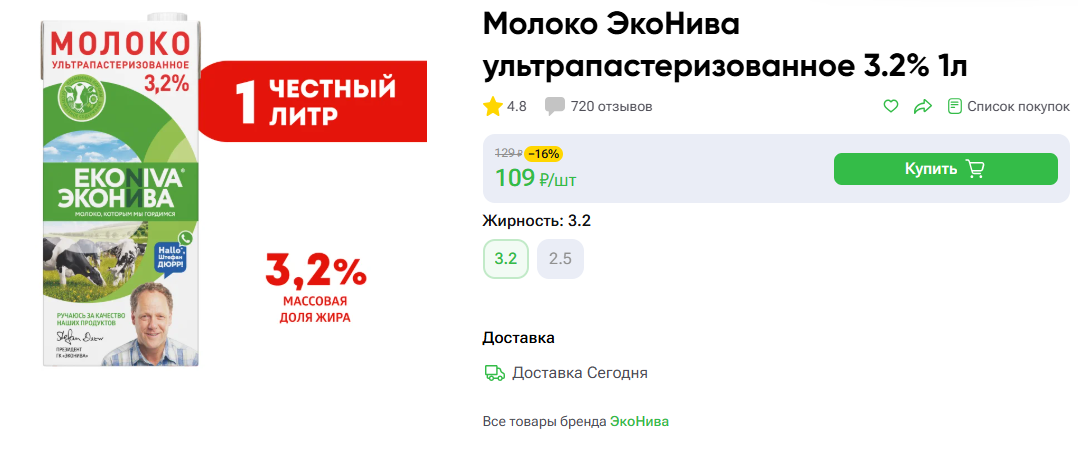
\includegraphics[width=\textwidth, keepaspectratio]{example_product}
	}
	\caption{Условный пример страницы с товаром}\label{fig:example_product}
\end{figure}


Собранные данные включали информацию о дате сбора, названии товара, единице измерения, цене продажи и старой цене в случаях, когда товар продавался со скидкой (пример собранной информации представлен в таблице~\ref{tab:product_data}). Наличие информации о  особенно важно, поскольку для построения индексов цен, согласно официальной методологии Росстата, учитываются только регулярные цены (т.е. не цены распродаж). Кроме того, тенденции в доле распродажных цен от общего числа цен могут служить важным индикатором общего макроэкономического состояния в стране~\cite{Nakamura2008}. 

\begin{table}[h!]
	\centering
	\caption{Пример структуры данных о товарах}
	\label{tab:product_data}
	\scriptsize
	\begin{tabular}{|c|c|p{4cm}|c|c|c|c|c|}
		\hline
		\textbf{id} & \textbf{date} & \textbf{site\_title} & \textbf{category\_id} & \textbf{site\_code} & \textbf{site\_unit} & \textbf{posted\_price} & \textbf{sale} \\ \hline
		0 & 28.10.2019 & Молоко ЭкоНива ультрапастеризованное 3.2\% 1л & 22 & globus & 1 шт. & 77.99 & 1 \\ \hline
		1 & 28.10.2019 & Печенье Любятово Мария традиционное 156г & 29 & globus & 1 шт. & 184.99 & 0 \\ \hline
		2 & 28.10.2019 & Чай чёрный Greenfield Earl Grey Fantasy, 25×2 г & 31 & globus & 1 уп. & 85.99 & 0 \\ \hline
		\vdots & \vdots & \vdots & \vdots & \vdots & \vdots & \vdots & \vdots \\ \hline
	\end{tabular}
\end{table}


Собранные данные охватывают 33 категории продовольственных товаров, 38 категорий непродовольственных товаров и 6 категорий услуг. Следует отметить, что в данном исследовании термин «категория» обозначает совокупность товаров или услуг определённого вида (например, «Печенье»). Термин «позиция» используется для обозначения конкретного представителя данной совокупности (например, «Печенье Merba Два шоколада 200~г»).

При отборе категорий мы ориентировались на фиксированный набор товаров и услуг, используемый Росстатом, которые имеют высокий спрос среди населения и являются значимыми индикаторами при определении минимального размера оплаты труда. Некоторая узость набора товаров и услуг по сравнению с индексом потребительских цен (ИПЦ) объясняется ограниченными ресурсами, доступными на момент запуска нами автоматизированного сбора данных.

Как было упомянуто ранее, мы собрали информацию о ценах на 33 категории продуктов питания, которые входят в условный (минимальный) набор товаров, регулярно фиксируемый Росстатом каждый месяц (см. таблицу \ref{tab:food_categories}). Этот набор включает основные продукты, потребляемые большей частью населения, и поэтому имеет высокую социальную значимость. В целом наибольшая полнота с точки зрения длины и непрерывности рядов данных отмечается для продовольственных категорий. Наш опыт показал, что многие базовые продовольственные товары остаются «на полке» в течение долгого времени и почти не подвержены временному отсутствию.

\begin{longtable}{p{0.5cm} p{3.5cm} p{3.5cm} p{3cm}} % Уменьшение ширины столбцов
	\caption{Перечень продовольственных категорий, составляющих условный (минимальный) набор продуктов питания Росстата} \label{tab:food_categories} \\
	\toprule
	\textbf{№ п/п} & \textbf{Название категории} & \textbf{Единица измерения} & \textbf{Вес (количество) товара в год} \\
	\midrule
	\endfirsthead
	
	\toprule
	\textbf{№ п/п} & \textbf{Название категории} & \textbf{Единица измерения} & \textbf{Вес (количество) товара в год} \\
	\midrule
	\endhead
	
	\endfoot
	
	\endlastfoot
	
	\footnotesize % Уменьшение размера текста на большее значение
	1   & Говядина (кроме бескостного мяса) & кг & 15 \\
	2   & Свинина (кроме бескостного мяса) & кг & 4 \\
	3   & Баранина (кроме бескостного мяса) & кг & 1,8 \\
	4   & Куры охлажденные и мороженые & кг & 14 \\
	5   & Рыба мороженая неразделанная & кг & 14 \\
	6   & Сельдь соленая & кг & 0,7 \\
	7   & Масло сливочное & кг & 1,8 \\
	8   & Масло подсолнечное & кг & 7 \\
	9   & Маргарин & кг & 6 \\
	10  & Молоко питьевое цельное пастеризованное 2,5 - 3,2\% жирности & л & 110 \\
	11  & Сметана & кг & 1,8 \\
	12  & Творог нежирный & кг & 10 \\
	13  & Сыры сычужные твердые и мягкие & кг & 2,5 \\
	14  & Яйца куриные & 10 шт. & 18 \\
	15  & Сахар-песок & кг & 20 \\
	16  & Мука пшеничная & кг & 20 \\
	17  & Хлеб из ржаной муки и из смеси муки ржаной и пшеничной & кг & 115 \\
	18  & Хлеб и булочные изделия из пшеничной муки 1 и 2 сортов & кг & 75 \\
	19  & Рис шлифованный & кг & 5 \\
	20  & Пшено & кг & 6 \\
	21  & Горох и фасоль & кг & 7,3 \\
	22  & Вермишель & кг & 6 \\
	23  & Картофель & кг & 150 \\
	24  & Капуста белокочанная свежая & кг & 35 \\
	25  & Морковь & кг & 35 \\
	26  & Огурцы свежие & кг & 1,8 \\
	27  & Лук репчатый & кг & 20 \\
	
\end{longtable}

\newpage % Переход на новую страницу

\noindent
\textbf{Продолжение таблицы \ref{tab:food_categories}:} \\

\begin{longtable}{p{0.5cm} p{3.5cm} p{3.5cm} p{3cm}} % Уменьшение ширины столбцов
	\toprule
	\textbf{№ п/п} & \textbf{Название категории} & \textbf{Единица измерения} & \textbf{Вес (количество) товара в год} \\
	\midrule
	\endfirsthead
	
	\toprule
	\textbf{№ п/п} & \textbf{Название категории} & \textbf{Единица измерения} & \textbf{Вес (количество) товара в год} \\
	\midrule
	\endhead
	
	\endfoot
	
	\endlastfoot
	
	\footnotesize % Уменьшение размера текста на большее значение
	28  & Яблоки & кг & 18,6 \\
	29  & Печенье & кг & 0,7 \\
	30  & Карамель & кг & 0,7 \\
	31  & Чай черный байховый & кг & 0,5 \\
	32  & Соль поваренная пищевая & кг & 3,65 \\
	33  & Перец черный (горошек) & кг & 0,73 \\
	
\end{longtable}

Всего в базе содержится 2257 уникальных товаров, цены на которые регистрировались в разные периоды. Самые длительные временные ряды начинаются с января 2019 года, а самые короткие — с июня того же года. Данные по продовольственным товарам охватывают период с 31 января 2019 года по 1 октября 2024 года. Непродовольстенные товары обладают в целом значительно меньшими периодами «жизни» на сайте и в выборке охватывают период с 12 февраля 2019 года по 2 июня 2022 года. Наконец, цены на услуги доступы за период с 18 февраля 2019 года по 30 июня 2022 года.

В начале сбора данных ежедневное количество уникальных позиций товаров и услуг составляло 546 позиций, в конце – 370 позиций. Максимальное число позиций, собираемых в день за рассматриваемый период, составило 2110 (рис.~\cref{fig:count_obs}).

\begin{figure}[ht]
	\centerfloat{
		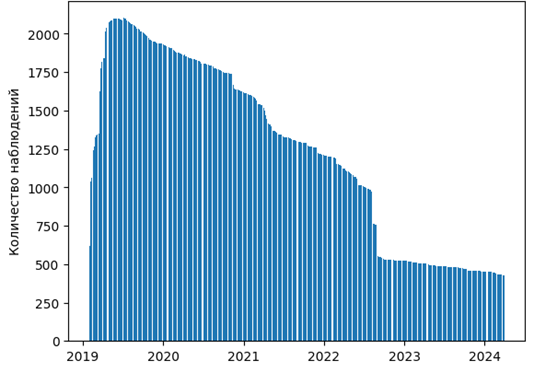
\includegraphics[scale=1]{count_obs}
	}
	\caption{Количество ежедневных наблюдений}\label{fig:count_obs}
\end{figure}

Поскольку сбор данных начался за год до начала пандемии COVID-19 и продолжается до настоящего времени, у нас есть возможность изучить отличительные характеристики различных периодов: острой фазы пандемии (первая половина 2020 года), постепенного снятия ограничений (2021 год), а также тенденции, произошедшие после введения ограничительных мер в отношении России в 2022 году.

Наличие информации о единице измерения товара позволило нам произвести дополнительную проверку того, насколько собираемые нами данные соответствуют динамике цен офлайн-ритейлеров. Так, наличие этой информации позволило рассчитать стоимость условного (минимального) набора продуктов по данным онлайн-ритейлеров и сопоставить ее со стоимостью аналогичного набора, стоимость которого отслеживается Росстатом по отдельным городам. Чтобы рассчитать стимость такого набора, мы брали 25 перцентиль стоимости внутри категории продуктов и умножали на норму потребления (табл.~ \ref{tab:food_categories}). Выбор 25 перцентиля объясняется тем, что Росстат рассматривает в своей статистике марки товаров, которые наиболее популярны среди населения, и, следовательно, собираемые данные по ценам на товары, вероятно, должны быть недорогими и доступными большинству людей.

На рисунке~\cref{fig:basket_plot} представлены графики стоимости таких наборов на основе данных по ценам онлайн-ритейлеров и данным, представленным на сайте Росстата для г. Москвы за период с 2019 по 2022 гг. Визуально динамика между стоимостями наборов является достаточно близкой, что можно объяснить следованием принципов сбора репрезентативных данных из работы \cite{cavallo2016billion}. Важную роль сыграл отбор преимущественно мультиканальных ритейлеров и ручной отбор конкретных марок продуктов, что позволило максимально приблизиться к официальной методологии Росстата.

Более формальным подтверждением наличия связи между наборами является оценка корреляции между стоимостями наборов. Значение этой оценки для очищенных от тренда рядов составила 0,82, что свидетельствует о наличии сильной линейной связи в динамике стоимостей наборов.

\begin{figure}[ht]
	\centerfloat{
		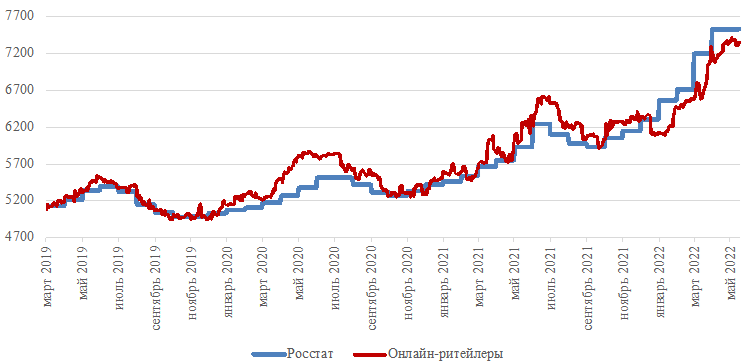
\includegraphics[width=\textwidth, keepaspectratio]{basket_plot}
	}
	\caption{Стоимость условного (минимального) набора продуктов по данным Росстата и онлайн-данным для г. Москвы (руб.)}\label{fig:basket_plot}
\end{figure}

Стоит отметить, что мы видим расхождение в динамике стоимостей наборов после марта 2020 года (и до, приблизительно, сентября) по сравнению с динамикой в 2019 году. Стоимость набора продуктов онлайн-ритейлеров стала расти существенно быстрее, чем стоимость набора по данным Росстата. Такое резкое удорожание объясняется введением локдауна в Москве и связанным с этим шоком спроса на доставку продуктов на дом. Таким образом, этот случай расходится с тем, что было получено в работе \cite{hillen2021covid}, где автор показала что существенного удорожания продуктов на данных Amazon Fresh после введения карантинных ограничений не произошло. 

\section{Анализ жесткости цен в онлайн-ритейле}\label{sec:ch3/sec2}

В данной главе будут рассмотрены стилизованные факты, касающиеся жесткости цен на данных онлайн-ритейлеров. Интерес представляет сопоставление результатов, полученных по г. Москве, с данными близких зарубежных исследований, а также сопоставление с жесткостью цен в традиционных офлайн-магазинах. Кроме того, будет рассмотрено сравнение жесткости цен в периоды относительной стабильности и нестабильности в российской экономике.

Следует сказать об основных показателях, которые нами будут использоваться в анализе. Основным показателем является частота изменения цен:
\begin{equation}
	\label{eq:equation_freq}
	f=\frac{m}{M},
\end{equation}
где \( m \) "--- число периодов, в которых цена изменялась, \( M \) "--- общее число периодов наблюдения.

Иным способом измерения жесткости цен является оценка дюрации, или периода неизменности цен. Дюрация - показатель, являющийся расчетным от частоты изменения цен и показывающий в течение какого времени цена на товар или услугу остается неизменной:
\begin{equation}
	\label{eq:equation_duration}
	D_k^{av}=\frac{-1}{ln⁡(1-F_k)},
\end{equation}
где \( k \) "--- идентификатор категории товара, \( F_k \) "--- средняя частота изменения. Показатель дюрации является более интерпретируемым, посколько показывает количество дней, в течение которых цена остается неизменной.

В таблице 11 представлены результаты оценки средней частоты изменения цен по используемой нами выборке с 2019 по 2022 гг. Средняя частота была рассчитана как доля изменённых цен от общего числа товаров внутри категории (в день). Анализ показывает значительную неоднородность частот между продовольственными, непродовольственными категориями товаров, а также среди отдельных категорий услуг. 

Среди продовольственных товаров (табл.~\ref{tab:products}) наиболее высокой частотой изменения цен характеризуются сезонные продукты. Так, для картофеля этот показатель составил в среднем 7,17\% в день, для огурцов — 6,75\%, яблок — 6,64\%, капусты — 4,98\%, моркови — 4,69\% и репчатого лука — 4,56\%. Сезонный характер предложения этих товаров приводит к их высокой волатильности и, как следствие, частым изменениям цен. 

\begin{longtable}{|p{1cm}|p{8.5cm}|p{3.5cm}|p{3cm}|} % Уменьшение ширины столбцов
	\caption{Средние частоты и дюрации: Продовольственные товары} \label{tab:products} \\
	\hline
	\textbf{№ п/п} & \textbf{Наименование категории} & \textbf{Средняя частота (\% в день)} & \textbf{Средняя дюрация (дней)} \\
	\hline
	\hline
	\endfirsthead
	
	\hline
	\textbf{№ п/п} & \textbf{Наименование категории} & \textbf{Средняя частота (\% в день)} & \textbf{Средняя дюрация (дней)} \\
	\hline
	\hline
	\endhead
	
	\hline
	\endfoot
	
	\hline
	\endlastfoot
	
	\footnotesize % Уменьшение размера текста на большее значение
	1   & Баранина (кроме бескостного мяса) & 1,13 & 88,0 \\
	2   & Говядина (кроме бескостного мяса) & 0,76 & 73,6 \\
	3   & Пшено & 1,73 & 57,3 \\
	4   & Рыба мороженая неразделанная & 1,97 & 50,3 \\
	5   & Горох и фасоль & 2,27 & 43,6 \\
	6   & Хлеб и булочные изделия из пшеничной муки 1 и 2 сортов & 2,32 & 42,6 \\
	7   & Свинина (кроме бескостного мяса) & 2,51 & 39,3 \\
	8   & Сахар-песок & 2,63 & 37,5 \\
	9   & Сыры сычужные твердые и мягкие & 2,81 & 35,1 \\
	10  & Рис шлифованный & 2,81 & 35,1 \\
	11  & Карамель & 2,92 & 33,7 \\
	12  & Сельдь соленая & 2,97 & 33,2 \\
	13  & Соль поваренная пищевая & 3,2 & 30,7 \\
	14  & Печенье & 3,29 & 29,9 \\
	15  & Вермишель & 3,59 & 27,4 \\
	16  & Маргарин & 3,59 & 27,4 \\
	17  & Куры охлажденные и мороженые & 3,6 & 27,3 \\
	18  & Крупа гречневая-ядрица & 3,63 & 27,0 \\
	19  & Мука пшеничная & 3,66 & 26,8 \\
	20  & Чай черный байховый & 3,69 & 26,6 \\
	21  & Перец черный (горошек) & 3,71 & 26,5 \\
	22  & Яйца куриные & 3,76 & 26,1 \\
	23  & Молоко питьевое цельное пастеризованное 2,5--3,2\% жирности & 3,86 & 25,4 \\
	24  & Масло сливочное & 3,88 & 25,3 \\
	25  & Творог нежирный & 3,92 & 25,0 \\
	26  & Хлеб из ржаной муки и из смеси муки ржаной и пшеничной & 3,98 & 24,6 \\
	27  & Сметана & 4,03 & 24,3 \\
	28  & Масло подсолнечное & 4,51 & 21,7 \\
	29  & Лук репчатый & 4,56 & 21,4 \\
	30  & Морковь & 4,69 & 20,8 \\
	31  & Капуста белокочанная свежая & 4,98 & 19,6 \\
	32  & Яблоки & 6,64 & 14,6 \\
	33  & Огурцы свежие & 6,75 & 14,3 \\
	34  & Картофель & 7,17 & 13,4 \\
	
\end{longtable}

Среди непродовольственных товаров (таб.~\ref{tab:non_food_products}) максимальная частота изменения цен наблюдается у лекарственных препаратов. Например, для корвалола она составила 8,84\%, а для анальгина — 7,22\%. Такая высокая частота изменений цен может быть связана как с сезонными вспышками простудных заболеваний, так и с эпидемическими волнами, провоцирующими резкий рост спроса на данные препараты.

\begin{longtable}{|p{1cm}|p{8.5cm}|p{3.5cm}|p{3cm}|} % Задаем ширину столбцов
	\caption{Средние частоты и дюрации: Непродовольственные товары}
	\label{tab:non_food_products} \\
	\hline
	\textbf{№ п/п} & \textbf{Наименование категории} & \textbf{Средняя частота (\% в день)} & \textbf{Средняя дюрация (дней)} \\
	\hline
	\hline
	\endfirsthead
	
	\hline
	\textbf{№ п/п} & \textbf{Наименование категории} & \textbf{Средняя частота (\% в день)} & \textbf{Средняя дюрация (дней)} \\
	\hline
	\hline
	\endhead
	
	\hline
	\endfoot
	
	\hline
	\endlastfoot
	
	35 & Джемпер для детей школьного возраста & 0,02 & 4 999,5 \\ \hline
	36 & Кроссовые туфли для детей с верхом из искусственной кожи & 0,06 & 1 666,2 \\ \hline
	37 & Брюки для детей школьного возраста из джинсовой ткани & 0,07 & 1 428,1 \\ \hline
	... & Добавьте остальные строки для непродовольственных товаров & ... & ... \\ \hline
	69 & Метамизол натрия (Анальгин отечественный) & 7,22 & 13,3 \\ \hline
	
\end{longtable}

Услуги (таб.~\ref{tab:services}), напротив, характеризуются сравнительно низкой частотой изменения цен. Это объясняется высокой долей трудовых издержек в их стоимости и более редким пересмотром цен трудовых контрактов по сравнению с сырьём.

\begin{longtable}{|p{1cm}|p{8.5cm}|p{3.5cm}|p{3cm}|} % Ширина столбцов оптимизирована
	\caption{Средние частоты и дюрации: Услуги}
	\label{tab:services} \\
	\hline
	\textbf{№ п/п} & \textbf{Наименование категории} & \textbf{Средняя частота (\% в день)} & \textbf{Средняя дюрация (дней)} \\
	\hline
	\hline
	\endfirsthead
	
	\hline
	\textbf{№ п/п} & \textbf{Наименование категории} & \textbf{Средняя частота (\% в день)} & \textbf{Средняя дюрация (дней)} \\
	\hline
	\hline
	\endhead
	
	\hline
	\multicolumn{4}{r}{Продолжение на следующей странице} \\
	\hline
	\endfoot
	
	\hline
	\endlastfoot
	
	71 & Постановка набоек & 0 &  \\ \hline
	72 & Стрижка модельная в женском зале & 0,06 & 1 666,2 \\ \hline
	73 & Абонентская плата за неограниченный объем местных телефонных соединений & 0,14 & 713,8 \\ \hline
	74 & Помывка в бане в общем отделении & 0,16 & 624,5 \\ \hline
	75 & Проезд в городском муниципальном автобусе & 0,30 & 332,8 \\ \hline
	76 & Проезд в троллейбусе & 0,32 & 312,0 \\ \hline
	
\end{longtable}


Еще одной важной характеристикой ценообразования онлайн-ритейлеров является средний размер изменения цен. Наш результат показал, что по абсолютной величине цены в среднем меняются на 6,7\%. 

\begin{figure}[h!]
	\centering
	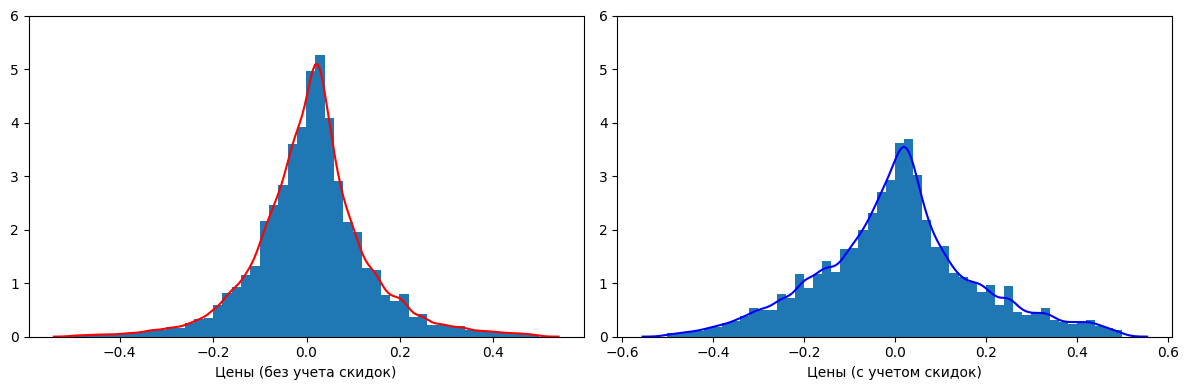
\includegraphics[width=\textwidth]{hist.png} % Укажите путь к вашему изображению
	\caption{Гистограмма и KDE для цен с учетом и без учета скидок}
	\label{fig:hist}
\end{figure}

В таблице \ref{tab:comparison} приведено сравнение наших оценок жесткости цен и среднего размера изменений цен с данными исследования \cite{cavallo2018scraped}, проведенного среди онлайн-ритейлеров США, Аргентины, Бразилии, Чили и Колумбии. Для обеспечения сопоставимости мы рассчитали среднюю продолжительность неизменности цен (дюрацию) на основе средней частоты изменения всех цен (включая распродажи) в наших еженедельных данных. Как видно из таблицы, оценка дюрации в России оказалась значительно ниже, чем в \cite{cavallo2018scraped}, что указывает на более частые изменения цен в России по сравнению с указанными странами. Это может быть связано с двумя факторами. Во-первых, в нашей выборке преобладают продовольственные товары, которые, как правило, меняются чаще, чем непродовольственные (см., например, \cite{bils2004some}). Во-вторых, в 2022 году (который включен в наши расчеты) в России наблюдался резкий рост инфляции, что также могло привести к увеличению частоты изменения цен по сравнению с зарубежными странами.

Кроме того, из таблицы видно, что средний размер изменений цен в России ниже, чем в сравниваемых странах. Это объясняется тем, что в исследуемый период инфляция в нашей выборке была относительно низкой, что позволяло ритейлерам изменять цены постепенно и на небольшие величины.

\begin{table}[h]
	\centering
	\small % Уменьшение размера шрифта
	\caption{Сопоставление результатов по средней дюрации и размеру изменений цен с зарубежными оценками из работы \cite{cavallo2018scraped}}
	\label{tab:comparison}
	\begin{tabularx}{\textwidth}{|X|X|X|X|X|X|X|} % Использование tabularx с шириной \textwidth
		\hline
		Показатель & Наши результаты за 2019–2022 гг. & \multicolumn{5}{c|}{Результаты \cite{cavallo2018scraped} за период с 2007 по 2010 гг.} \\
		\cline{3-7}
		&  & США & Аргентина & Бразилия & Чили & Колумбия \\
		\hline
		Дюрация (среднее, недель) & 1,1 & 2,9 & 2,4 & 1,5 & 2,9 & 2,0 \\
		\hline
		Средний размер изменений по модулю & 6,7 & 22,0 & 12,2 & 11,5 & 14,7 & 10,7 \\
		\hline
	\end{tabularx}
\end{table}

% частота изменения цен - общая и по отдельным товарам - продам, непродам и услугам
% можно сразу написать о том, какие результаты были получены на зарубежных исследованиях по онлайн-ценам - Lunneman, Wintr 2011, Cavallo 2018
%% описать показатели жесткости цен
% 

Отдельного внимания заслуживает наличие сезонности в изменениях цен. Такая сезонность может иметь значение для мер воздействия денежно-кредитной политики на экономику. Так, в работе \cite{olivei2007} было показано, что реакция выпуска на монетарные шоки, идентифицированные с помощью структурной VAR-модели, оказывается сильнее для шоков, происходящих в первом и втором кварталах, по сравнению с шоками, происходящими в третьем и четвертом кварталах. Эмпирические данные по США потверждают эти выводы: так, в работе \cite{Nakamura2008} на месячных данных авторы рассчитали, что частота изменения цен в первом квартале составляет 15,9\%, но снижается до всего лишь 8,2\% в четвертом квартале. Для цен производителей большая часть сезонности объясняется резким скачком частоты изменения цен в январе. В работе \cite{alvarez2006sticky} обнаруживают схожие закономерности для потребительских цен в зоне евро.

Наши результаты (рис. \ref{fig:seasonality}) показывают, что наибольшая доля изменений приходится на второе полугодие, а именно на ноябрь-декабрь. Во многом такое поведение ритейлеров объясняется количеством изменений цен, ассоциированных с распродажами и связанными с этим подстройками цен для более эффективной конкуренции.

\begin{figure}[h]
	\centering
	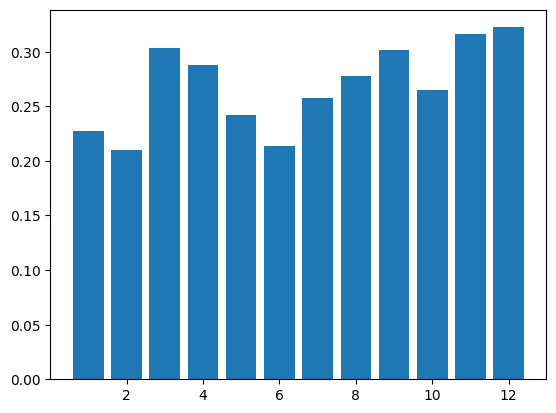
\includegraphics[width=0.8\textwidth]{seasonality.png} % Укажите путь к изображению и настройте ширину
	\caption{Частота изменения цен по месяцам} % Подпись к изображению
	\label{fig:seasonality} % Метка для ссылок в тексте
\end{figure}
 



